% !Mode:: "TeX:UTF-8" 

\BiChapter{感知融合}{3}\label{chpt-perceptron}
\BiSection{感知模型}{}
\BiSubsection{目标识别模型}{}
本文使用YOLO系列模型作为本次目标识别模型,分别尝试了YOLOv5\upcite{YOLOv5}和YOLOv8\upcite{YOLOv8}作为目标识别器,
下面分别对其模型架构改进进行介绍:

YOLOv5主要是对YOLOv4\upcite{YOLOv4}模型进行了少许改进,YOLOv4模型在Backbone部分(初步特征提取)的主要改进
是使用了基于跨阶段部分网络(Cross Stage Partial Networks, CSPNet)\upcite{CSPNet}
结构的DarkNet\upcite{YOLOv3}并在输出特征时使用空间金字塔池化(Spatial Pyramid Pooling,SPP)\upcite{SPP}对特征进行不同尺度上的提取,
在Neck部分(进一步特征提取)中使用了路径聚合网络(Path Aggregation Network, PANet)\upcite{PANet},结合特征金字塔与路径压缩,
缩短了较低层与最顶层特征之间的信息路径,能够有效进行特征融合。

而YOLOv8模型结构上仍然使用CSP和SPP进行特征提取,相对YOLOv5使用了更多的工程优化方法对模型预测速度进行大幅优化,
Head部分(预测框输出)则重新回到YOLOv1\upcite{YOLO}无锚框预测的方法,使预测框不再受到锚框约束。

ByteTrack\upcite{ByteTrack}是一种基于Kalman滤波的多目标跟踪(Multiple Object Tracking, MOT)算法,
首先需要分别对不同边界框作为跟踪对象,建立独立的线性运动方程,通过Kalman滤波结合之前帧的追踪信息,
以递归的方式给出目标边界框在当前时刻下的位置预测,再通过计算交并比(定义~\ref{def-iou})定位当前帧下跟踪对象的位置。
与传统MOT算法不同的是,
ByteTrack尝试利用滤波预测的方法,从更低的置信度对应的边界框中找到可能被忽略的跟踪边界框,
从而恢复可能因遮挡等原因被低估的边界框。

\BiSubsection{光学字符识别模型}{}
PaddleOCR\upcite{PPOCR}是百度公司研发并开源的一个基于PaddlePaddle框架的光学字符识别(Optical Character Recognition, OCR)
系统,PaddleOCR提供了一整套从图像预处理到文字识别的方案,其模型架构主要分为如下两个模块:
\begin{enumerate}
  \item 文本检测模块:使用ResNet\upcite{ResNet}、MobileNet\upcite{MobileNet}等经典的卷积神经网络作为特征提取网络,使用特征金字塔网络(Feature Pyramid Networks,FPN)\upcite{FPN}等方法来融合多尺度特征,
  使用可微分二值化(Differentiable Binarization,DB)\upcite{DB}等方法来预测文本框。
  \item 文本识别模块:使用卷积循环神经网络(Convolutional Recurrent Neural Networks, CRNN)\upcite{CRNN}提取文字区域的特征,
  首先使用卷积网络对图像进行特征提取,再使用Bi-LSTM\upcite{BiLSTM}等序列模型来捕捉字符之间的依赖关系,
  最后使用CTC(Connectionist Temporal Classification)\upcite{CTC}作为文字序列的损失函数。
\end{enumerate}

\BiSubsection{图像分类模型}{}
本毕设的图像分类模型使用ResNet结构,其核心思想是通过引入短连接(Shortcut Connections),
使得网络可以直接学习残差(Residual),从而更容易学习到恒等映射,
缓解深度神经网络中梯度消失的问题。具体来说,ResNet使用残差块(Residual Block)来实现上述操作,
残差块两部分构成,卷积层:卷积变换$F_W(\cdot)$、批归一化(Batch Normalization, BN)\upcite{BN}以及ReLU激活函数;
残差连接:将输入直接加在卷积层的输出结果上。残差块结构可以表示为
\begin{equation}
  y = \sigma(\text{BN}(F_W(x))) + x
\end{equation}
其中$x$为输入图像特征,$y$为输出图像特征,$F_W$是以卷积核$W$的卷积变换,BN为批归一化操作,$\sigma(x)=\frac{x+|x|}{2}$为ReLU函数。

\BiSection{感知特征提取}{}
在感知特征提取中,本文将同时用到上述三种模型作为一阶段图像特征提取,分别可以得到当前时刻下三个预处理信息:
剩余时间(OCR)、竞技场中的预测框(YOLO)、当前手牌及总圣水(图像分类器)。
下面将介绍特征提取器的设计方法,可以将预处理信息进一步转化为决策模型的输入信息,它们分别为
环境状态信息提取(State)、执行动作信息提取(Action)和环境奖励信息提取(Reward)。
\begin{wrapfigure}[15]{r}{.5\textwidth} % 文字环绕行数为13行, 图片靠右 (l为靠左), 图片占0.5的行宽
  \centering
  \vspace{-1ex}
  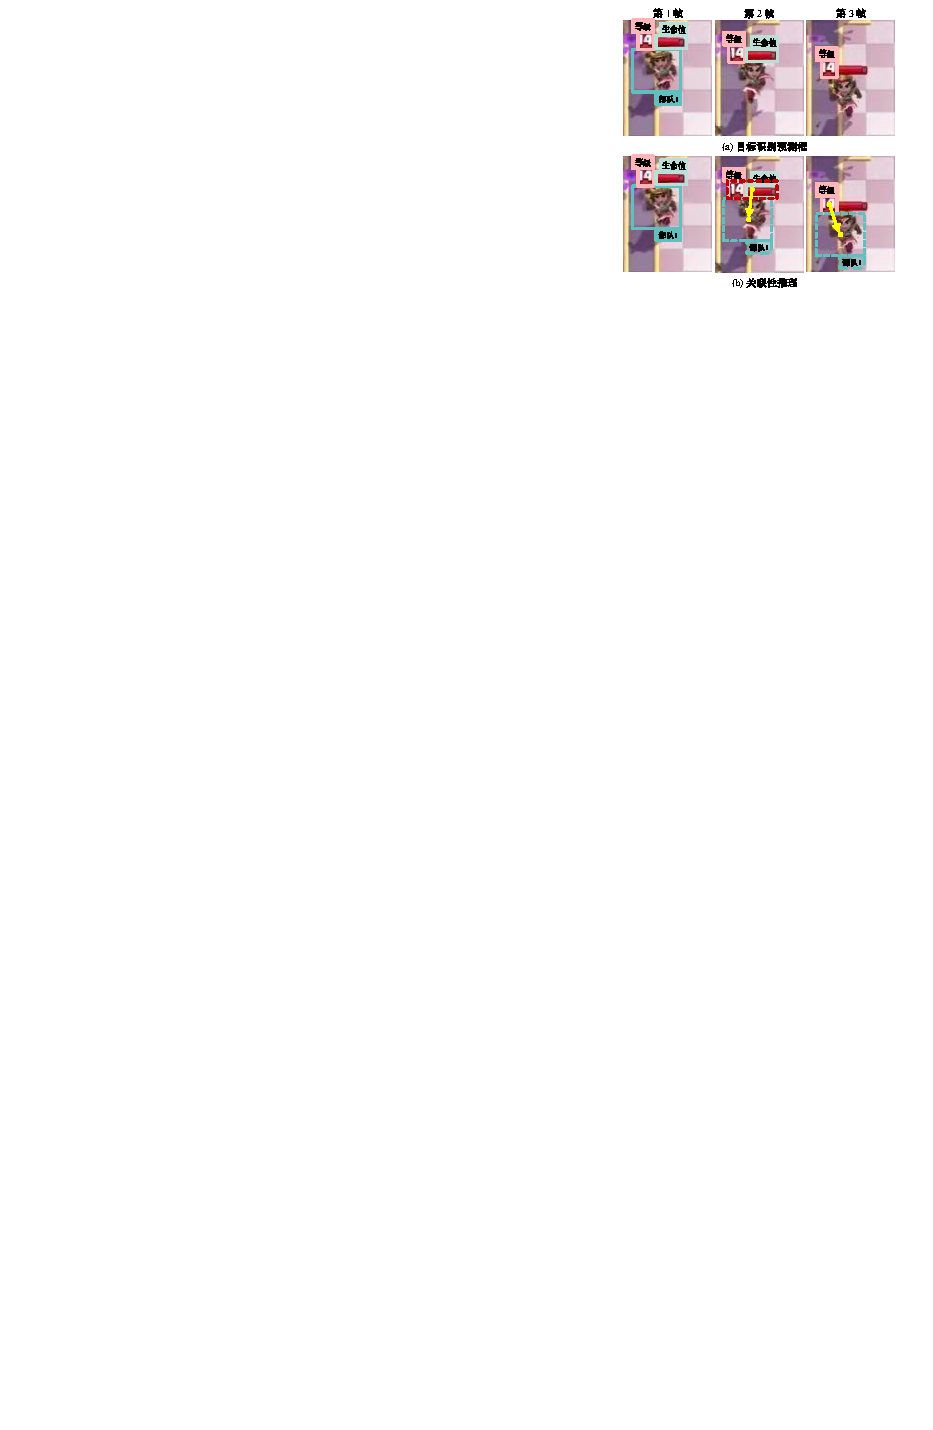
\includegraphics[width=.5\textwidth]{perceptron_improve.pdf}
  \caption{当模型在第1帧关联了部队1与等级、生命值信息的对应关系,通过目标追踪及上下文信息记忆,
  即使在第2,3帧未能目标识别模型未能检测到部队1,通过等级或生命值的关联性推理,模型同样可以推理得到当前单位的真实位置。}
  \label{fig-state-connect}
\end{wrapfigure}
\vspace{-4ex}
\BiSubsection{状态特征提取}{}
状态特征包括四种信息:
\begin{itemize}
  \item 经过的总时长:直接通过OCR对图~\ref{fig-introduction}~右上角的阶段剩余时间信息识别后,简单处理即可。
  \item 竞技场中部队信息:每个部队由五个参数构成二维位置坐标、类别、派别、生命值、其余条状信息构成
  $u:=(\boldsymbol{x}, \text{cls}, \text{bel}, \text{bar}_1, \text{bar}_2)$。
  \item 手牌信息:由于手牌可以被拖出但不释放,因此仅识别手牌图像无法确定其真实状态,
  需要通过是否做出动作来判断当前手牌是否被使用,
  故要基于动作特征~\ref{sub-sec-action}~来判断当前真实手牌信息。
  \item 圣水信息:通过OCR对图~\ref{fig-introduction}~下方可用圣水中的数字进行识别。
\end{itemize}
% 这里一定要空一行

在竞技场中部队信息特征提取时,本文引入一种基于上下文关联性推理的方式来解决部队识别错误或漏识别的问题,
在本任务中由于等级和生命值信息容易识别,每个部队都存在一个与之唯一对应的等级和生命值信息,
且部队与等级或生命值信息的相对位置基本不变,所以当部队识别框消失、类别识别错误、派别识别错误时,
利用之前与之关联的等级和生命值信息中进行修正,实现效果如图~\ref{fig-state-connect}~所示。
\vspace{-3.5ex}
\begin{wrapfigure}[11]{r}{.6\textwidth} % 文字环绕行数为13行, 图片靠右 (l为靠左), 图片占0.5的行宽
  \centering
  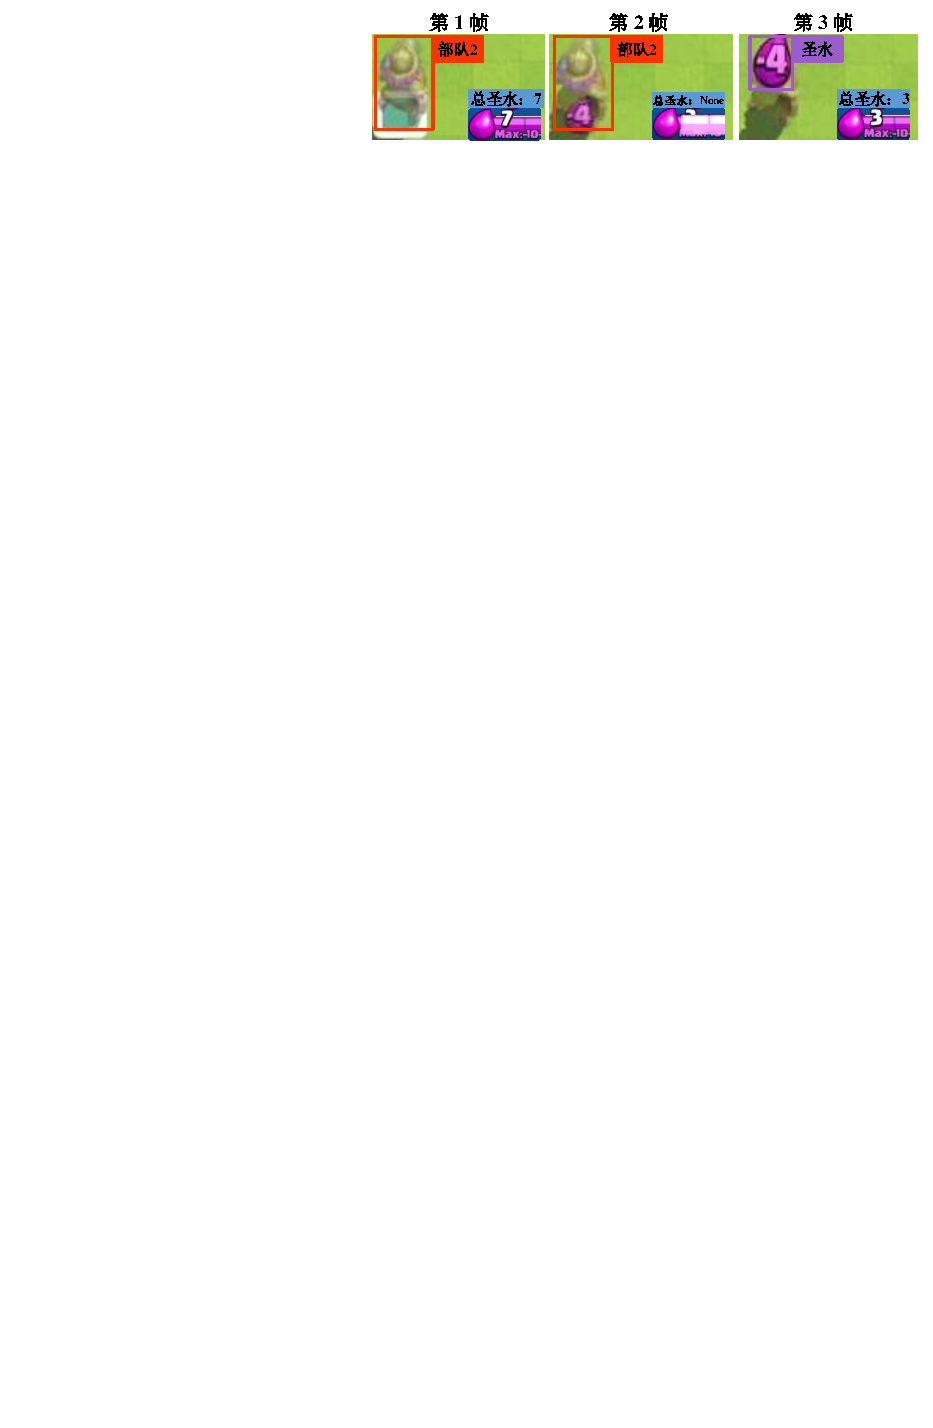
\includegraphics[width=.6\textwidth]{state_and_action.pdf}
  \caption{动作直接导致的错误状态先验信息:第1帧中目标识别错误识别到未部署的部队状态;
  第2帧中OCR识别器在目标识别识别到动作之前,产生了错误的总圣水识别信息,因此需要将动作帧提前到该帧之前;
  第3帧中目标识别成功识别到圣水动画,可以判断玩家在该时刻之前部署了部队。}
  \label{fig-state-action}
\end{wrapfigure}

需要注意状态处理的细节问题,在执行动作之前,状态特征中应不包含任何直接与该动作相关的先验信息,
否则模仿学习可以通过该先验信息直接给出动作预测,而真实环境中由于不再出现这类动作的先验信息,
所以导致模型无法做出决策,错误状态信息如右图~\ref{fig-state-action}~所示。

假设目标识别每个预测框的识别结果包括七个参数$b:=(x,y,w,h,\text{id},\text{cls},\text{bel})$,
分别为预测框的中心点$(x,y)$,宽高$(w,h)$,目标追踪编号id,预测所属类别cls以及所属派别bel。

\begin{definition}[计数记忆缓存]
  设$I\subset \mathbb{N}$为目标追踪指标集,$S$为可数记忆元素集合,$V\subset \mathbb{R}^+$为可用时间集合,
  定义$M_{T}:I\times S\to\mathbb{Z}^+\times V$为缓存大小为$T$的计数记忆缓存,其满足
  $\forall~ \text{id}\in I, s\in S, (n,t):=M_T(\text{id},s)$,在时间间隔$[t-T,t]\cap V$下追踪指标为id的预测框中,
  存在$n$个预测框包含元素$s$。
\end{definition}

初始化派别记忆缓存$M_{T}^{\text{bel}}$和类别记忆缓存$M_{T}^{\text{cls}}$,其记忆元素集合分别为派别集合$\{0,1\}$
及全体类别集合,假设当前时间为$t$,于是状态特征提取可以分为下述6步\footnote{状态特征提取部分代码见附录~\ref{app-state-feature}~。}:

1. 更新派别记忆缓存:对当前每个预测框$b$,更新$M_{T}^{\text{bel}}(b^{\text{id}}, b^{\text{bel}})$,并对$b^{\text{bel}}$进行修正,
使得$M_T^{\text{bel}}(b^{\text{id}}, b^{\text{bel}})_1 = \max\left\{M_T^{\text{bel}}(b^{\text{id}},x)_1:x\in\{0,1\}\right\}$。

2. 全局文本信息查找:使用OCR对当前竞技场中全部文本信息进行识别,用于解决图~\ref{fig-state-action}~中未放置单位的错误识别问题。

3. 等级、生命值及防御塔信息关联:将等级与部队生命值、防御塔与防御塔生命值进行关联。

4. 部队信息关联:基于贪心的关联策略,从下至上,将部队与在一定范围内最近的等级和生命值进行关联,并基于步骤2结果,去除具有对应文本的部队单位。

5. 缓存清理:将$M_T^{\text{bel}},M_T^{\text{cls}}$中超出时间间隔$[t-T,t]$的信息置零。

6. 更新类别记忆缓存:结合关联性信息,对部队及其关联的等级和生命值信息所对应的$M_T^{\text{cls}}$进行更新,同时对部队类别进行修正,
更新及修正方法与步骤1类似。

\BiSubsection{动作特征提取}{}\label{sub-sec-action}
动作特征包含两种信息:
\begin{itemize}
  \item 当前执行动作的二维坐标$\bd{x}$。
  \item 当前执行动作所用的卡牌编号$\text{card}\in\{1,2,3,4\}$。
\end{itemize}

在进行动作特征提取时,需通过目标识别模型识别到的圣水预测框来判断执行动作的时刻以及坐标位置,
对圣水预测框的目标检测如图~\ref{fig-state-action}~中第3帧所示,但是在第2帧中已经出现了圣水对象,
动作执行本应该发生在第2帧,但是模型无法对其进行识别导致动作判断出现延迟,
所以需通过第2帧中总圣水识别发生突变来进行判断动作的执行,因此需要将第3帧识别到的动作前移至第2帧上。

还需结合当前手牌及圣水上方的文字信息来判断使用的卡牌编号,通过维护一个手牌记忆缓存记录当前可用手牌,
当手牌被玩家或智能体拖出牌库,则将其加入到候选手牌中,每次动作执行的卡牌编号将文本与候选手牌进行比对得到,
当两个文本串的Levenshtein编辑距离\upcite{LevenshteinDistance}不超过2时,则认为两个文本串相同。

初始化圣水记忆缓存$M_{T}^{\text{elixir}}$,其记忆元素集合为可部署单位的二维坐标空间,假设当前时间为$t$,
于是动作特征提取可以分为下述4步\footnote{动作特征提取部分代码见附录~\ref{app-action-feature}~。}:

1. 缓存清理:将$M_{T}^{\text{elixir}}$中超出时间间隔$[t-T,t]$的信息置零。

2. 更新可用手牌及候选手牌:通过手牌分类器的识别结果以及缓存中记录的手牌,可以完成候选手牌、可用手牌的信息更新。

3. 记录总圣水的突变时刻:通过OCR识别当前总圣水以及上一帧总圣水,可用判断当前的总圣水是否发生减少或者无法识别的情况,
当此类情况发生则认为动作执行可能发生在当前帧。

4. 动作查找:通过竞技场中对圣水单位的目标识别,判断动作执行的位置,动作执行的真实时刻为一段时间内最早发生的总圣水突变时刻,
动作卡牌编号需要结合OCR文本识别与候选手牌集合判断,最后再对当前可用手牌进行更新。
\BiSubsection{奖励特征提取}{}
奖励特征仅包含奖励$r\in\mathbb{R}$一种信息,通过OCR识别可以得到敌我防御塔具体生命值,敌我主、副塔如图~\ref{fig-introduction}~中所示,
设$h_{i}^{\text{bel}}, (i\in\{0,1,2\},\text{bel}\in\{0,1\})$为防御塔生命值,
当$i=1,2$时表示左右两个副塔生命值,$i=0$表示主塔生命值,$\text{bel}=0,1$分别表示我方和敌方建筑,
$\Delta h_{i}^{\text{bel}}$表示前一帧与当前帧生命值的差值,$H_{i}^{\text{bel}}$表示对应防御塔的总生命值,分别定义如下四种奖励函数:

1. 防御塔生命值奖励
\begin{equation}
  r_{tower} = \sum_{\text{bel}=0}^1\sum_{i=0}^2(-1)^{\text{bel}+1}\frac{\Delta h_{i}^{\text{bel}}}{H_{i}^{\text{bel}}}
\end{equation}

2. 防御塔摧毁奖励$r_{distory}$:当敌我副塔被摧毁时给予$(-1)^{\text{bel}+1}$奖励,敌我主塔被摧毁时给予前者的$3$倍奖励。

3. 主塔激活奖励$r_{activate}$:当副塔均存活的条件下,主塔第一次失去生命值时,给予$(-1)^{\text{bel}}~0.1$奖励。

4. 圣水溢出惩罚$r_{elixir}$:当总圣水持续保持溢出状态时,每间隔$1$秒产生一次$0.05$的惩罚。

综合上述奖励,得到总奖励:
\begin{equation}\label{eq-reward}
  r = r_{tower} + r_{destory} + r_{activate} + r_{elixir}
\end{equation}

需要注意的是,当图像中的数字信息出现噪声干扰或产生错误目标位置识别时,需要终止奖励的错误更新,
例如:部署单位时其他部件对其产生的遮挡(等级、生命值、圣水、时钟、文本)
\footnote{奖励特征提取部分代码见附录~\ref{app-reward-feature}~。}。
